\chapter{Estadística descriptiva}

\section{Medidas de tendencia central}

\paragraph{\'Indice y subíndices}
El símbolo $X_{j}$ representa cualquiera de los  valores $X_{1},X_{2},X_{3},...$ que puede tomar la variable discreta $X.$


El símbolo $j$ denota cualquiera de los números naturales $1,2,3,...$ y se le llama \emph{índice} (o a veces \emph{subíndice} o también \emph{contador}).




\begin{defn}[Sumatoria]
\begin{align}
\sum_{j=1}^{N}X_{j}=X_{1}+...+X_{N}
\end{align}
\end{defn}



\begin{ejemplo}
 \begin{itemize}
  \item $\displaystyle \sum_{k=1}^{N}X_{k}Y_{k}=
  X_{1}Y_{1}+...+X_{N}Y_{N}$
  \item $\displaystyle \sum_{i=1}^{N} aX_{i}=
  aX_{1}+...+aX_{N}=a\sum_{n=1}^{N}X_{n}.$
 \end{itemize}

\end{ejemplo}



\begin{rem}
 Cuando se \emph{sobrentiende} que el contador $j$ \emph{corre} sobre los números $1,2,...,N,$ escribimos $\sum X_{j}$ o simplemente $\sum X$ en lugar de $\sum_{j=1}^{N}.$
\end{rem}


\paragraph{Linealidad}
\begin{problema}
 Si $a,b$ son constantes, demuestre que
 \begin{align}
\sum \left( aX+bY \right)=a\sum X + b\sum Y.
\end{align}
\end{problema}

\paragraph{Promedio}
UN \emph{promedio} es un valor representativo de un conjunto de datos que tiende a encontrarse en el centro de dicho conjunto. 

Por esta razón, también se le conoce como \emph{medidas de tendencia central.}



Se pueden definir varios tipo de promedios: 
\begin{itemize}
 \item Media aritmética;
 \item mediana;
 \item moda;
 \item media geométrica;
 \item media armónica.
\end{itemize}



 \begin{rem}
  Cada medida de tendencia central tiene ventajas y desventajas de acuerdo al tipo de datos y el propósito del uso.
 \end{rem}



\begin{defn}[Media aritmética]
 \begin{align}
 \label{3.1}
\bar{X} =\dfrac{X_{1}+...+X_{N}}{N} = \dfrac{\sum_{j=1}^{N}X_{j}}{N}=\dfrac{\sum X}{N}
\end{align}
\end{defn}



\begin{ejemplo}
 La media aritmética de $8,3,5,12,10$ es...
\end{ejemplo}



Si los números $X_{1},X_{2},...,X_{k}$ se presentan con \emph{frecuencias} $f_{1}, f_{2},...,f_{k}$ respectivamente su media aritmética es
\begin{align}
 \label{3.2}
 \bar{X}=\dfrac{f_{1}X_{1}+...+f_{k}X_{k}}{f_{1}+...+f_{k}}=\dfrac{\sum fX}{\sum f}=\dfrac{\sum fX}{N}.
\end{align}
dónde $N=\sum f$ es la \emph{suma de frecuencias} o \emph{total de casos.}


\begin{ejemplo}
 Si $5,8,6,2$ se presentan con frecuencias $3,2,4,1$ respectivamente, su media aritmética es...
\end{ejemplo}


\paragraph{Media aritmética ponderada}
Algunas veces, a los números $X_{1},...,X_{k}$ se les asignan ciertos \emph{factores de ponderación} o \emph{pesos} $w_{1},...,w_{k},$ tales que \begin{align}
\begin{cases}
0\% \leq w_{i}\leq 100\% \\
 \sum w_{i} = 100\%
\end{cases}
\end{align}


 \begin{defn}[Media ponderada]
  Si $w_{1},..,w_{k}$ son \emph{pesos} tales que $0\leq w_{i}\leq 1$ y $\sum w_{i}=1,$ entonces la correspondiente media (aritmética) ponderada de los números $X_{1},...,X_{k}$ es
  \begin{align}
\bar{X}= \dfrac{w_{1}X_{1}+...+w_{k}X_{k}}{w_{1}+...+w_{k}}=\dfrac{\sum wX}{\sum w}=\sum wX.
\end{align}
 \end{defn}



\begin{ejemplo}
 Si en una clase, al examen final se le da el triple del valor que a los exámenes parciales y un estudiante obtiene 85 en el final y 70 y 90 en los dos exámenes parciales, obtener su media ponderada.
\end{ejemplo}



\begin{enumerate}
 \item Si $w_{i}=\frac{1}{N},$ obtenemos la media aritmética usual. 
 \item Si $w_{i}=\frac{f_{i}}{N},$ obtenemos la fórmula \eqref{3.2}.
\end{enumerate}



%%%%%%%%%%%%%%
 \subsection{Datos agrupados}
 
 Cuando los números son muy grandes, se suele utilizar un pivote $P:$ 
 $$
 \bar{X}=P+\dfrac{\sum f_{i}d_{i}}{N},
 $$
 donde $d_{i}=X_{i}-P.$

 En ocasiones, utilizaremos la notación
 \begin{align}
 \bar{d}=\dfrac{\sum f_{i}d_{i}}{N},
 \end{align}
 de manera que $\bar{d}$ es la \emph{desviación promedio} y $\bar{X}=P+\bar{d}.$

 
 
 \begin{rem}

 Para datos agrupados, $X_{i}$ se escoge como la marca de la $i-$ésima clase.
 \end{rem}

 
 \paragraph{La mediana}
  La mediana $\til{X}$ de un conjunto de números acomodados en un orden de magnitud (es decir, en una ordenación) es el valor central o la media de dos valores centrales.
 
 
  \begin{ejemplo}
   \begin{itemize}
    \item La mediana de la lista de números $3,4,5,6,8,8,8,10$ es... 
    \item La mediana de la lista de números $5,5,7,9,11,12,15,18$ es..
   \end{itemize}

  \end{ejemplo}

 
 
  \begin{defn}[Mediana para datos agrupados]
   \begin{align}
    \texttt{Mediana}=L+\left(
    \dfrac{ \dfrac{N}{2}-\sum_{{C<C_{M}}}f}{f_{C_{M}}}
    \right)
   \end{align}
   donde 
   \begin{itemize}
    \item $L$ es la frontera inferior de la clase mediana, es decir, de la clase que contiene la mediana;
    \item $N$ es la frecuencia total; 
    \item $\sum_{{C<C_{M}}}f$ suma de las frecuencias de todas las clases anteriores a la clase mediana; 
    \item $f_{C_{M}}$ es la frecuencia de la clase mediana.
   \end{itemize}

  \end{defn}

 
 \paragraph{Moda}
  La moda de una lista de números es un valor que se presenta con la mayor frecuencia $f>1$.  \emph{La moda no es necesariamente existe ni es única.}
 
 
  \begin{ejemplo}
   \begin{itemize}
    \item La moda de la lista $2,2,5,7,9,9,9,10,10,11,12,18$ es...  En este caso, diremos que la lista es \emph{unimodal.}
    \item ?`Cuál es la moda de la lista $3,5,8,0,12,15,16$? 
    \item ?`Cuál es la moda de la lista $3,8,8,8,15,15,15$?  En este caso diremos que la lista es \emph{bimodal.}
   \end{itemize}

  \end{ejemplo}

 
 
  \begin{defn}[Moda para datos agrupados]
   \begin{align}
    \texttt{Moda}=
    L + \left( \dfrac{\Del_{1}}{\Del_{1}+\Del_{2}} \right)c
   \end{align}
 donde 
 \begin{enumerate}
  \item $L:$ Frontera inferior de la clase modal, es decir, de la clase que contiene la moda.
  \item $\Del_{1}:$ Exceso de frecuencia modal sobre la frecuencia en la clase inferior inmediata. 
  \item $\Del_{2}:$ Exceso de frecuencia modal sobre la frecuencia en la clase superior inmediata. 
  \item $c:$ Amplitud del intervalo de la clase modal.
 \end{enumerate}

  \end{defn}

 
 %%%%%%%%%%%%%%%%%%5
 %%%%%%%%%%%%%%%%%%%%%5

\subsection{Python}

\begin{lstlisting}[language=Python]
 numpy.mean(a, axis=None, dtype=None, out=None,
  keepdims=<class numpy._globals._NoValue>)
\end{lstlisting}

Calcula  la media aritmética sobre los elementos de un arreglo. \footnote{\href{https://github.com/numpy/numpy/blob/v1.13.0/numpy/core/fromnumeric.py\#L2806-L2909}{https://github.com/numpy/numpy/blob/v1.13.0/numpy/core/fromnumeric.py\#L2806-L2909}}


[]{Ejemplos}
 \begin{lstlisting}[language=Python]
a = np.array([[1, 2], [3, 4]])
print np.mean(a)
#2.5
print np.mean(a, axis=0)
#array([ 2.,  3.])
print np.mean(a, axis=1)
#array([ 1.5,  3.5])
\end{lstlisting}


[]{numpy.median}
 \begin{lstlisting}[language=Python]
  numpy.median(a, axis=None, out=None,
  overwrite_input=False, keepdims=False)
\end{lstlisting}

 Calcula la mediana de los elementos de un arreglo de números.\footnote{\href{https://docs.scipy.org/doc/numpy/reference/generated/numpy.median.html}{https://docs.scipy.org/doc/numpy/reference/generated/numpy.median.html}}


[,]{Ejemplos}
 \begin{lstlisting}[language=Python]
import numpy as np

a = np.array([[10, 7, 4], [3, 2, 1]])
print a
#array([[10,  7,  4],6[ 3,  2,  1]])
print np.median(a)
#3.5
print np.median(a, axis=0)
#array([ 6.5,  4.5,  2.5])
print np.median(a, axis=1)
#array([ 7.,  2.])

m = np.median(a, axis=0)
out = np.zeros_like(m)
print np.median(a, axis=0, out=m)
#array([ 6.5,  4.5,  2.5])
print m
#array([ 6.5,  4.5,  2.5])
b = a.copy()
print np.median(b, axis=1, overwrite_input=True)
#array([ 7.,  2.])

assert not np.all(a==b)
b = a.copy()
print np.median(b, axis=None, overwrite_input=True)
#3.5
assert not np.all(a==b)
\end{lstlisting}


\paragraph{\text{SciPy}}
SciPy es una biblioteca open source de herramientas y algoritmos matemáticos para Python...

SciPy contiene módulos para optimización, álgebra lineal, integración, interpolación, funciones especiales, FFT, procesamiento de señales y de imagen, resolución de ODEs y otras tareas para la ciencia e ingeniería. Está dirigida al mismo tipo de usuarios que los de aplicaciones como MATLAB, GNU Octave, y Scilab.\footnote{\href{https://es.wikipedia.org/wiki/SciPy}{https://es.wikipedia.org/wiki/SciPy}}

[, ]{Moda}
\begin{lstlisting}[language=Python]
import numpy as np
from scipy import stats

a = np.array([3,5,6,5,6,5,6,6,3,1,5])
print stats.mode(a)
# ModeResult(mode=array([5]), count=array([4]))
\end{lstlisting}

\begin{lstlisting}[language=Python]
b = np.array([[6, 8, 0, 0],
               [3, 3, 0, 3],
               [8, 1, 8, 5],
               [5, 3, 0, 5],
               [4, 7, 5, 3]])

print stats.mode(b)
# ModeResult(mode=array([[3, 3, 0, 3]]),
 count=array([[1, 2, 3, 2]]))
\end{lstlisting}

\begin{lstlisting}[language=Python]
print stats.mode(b, axis=1)
# ModeResult(mode=array([[0],[3],[8],[5],[3]]),
#           count=array([[2],[3],[2],[2],[1]]))

print stats.mode(b, axis=None)
# ModeResult(mode=array([3]), count=array([5]))
\end{lstlisting}
 
%
 \begin{problema} \label{problema:3.1}
  Escribir los términos de cada una de las siguientes sumas:
  \begin{enumerate}[(a)]
    \item $\displaystyle\sum_{j=0}^{6}X_{j}=$ 
    \item $\displaystyle\sum_{k=1}^{4}\left( Y_{k}-3 \right)^{2}=$ 
   \item $\displaystyle\sum_{k=1}^{N}a=$ 
   \item $\displaystyle\sum_{n=2}^{5}{f_{n}}X_{n}= $ 
   \item $\displaystyle\sum_{m=0}^{3}\left( X_{m}-a \right)=$
  \end{enumerate}
%
%
 \end{problema}
%
 
 
  \begin{problema}
   \label{problema:3.10}
   De 100 números, 20 fueron 4, 40 fueron 5, 30 fueron 6 y los restantes fueron 7. Encuentre su media aritmética.
  \end{problema}

 

 
  \begin{problema}
   \label{problema:3.13}
   Los pesos medio de cuatro grupos de estudiantes que constan de 15, 20, 10 y 18 individuos son 162, 148, 153 y 140 libras, respectivamente. Encuentre el peso medio de todos los estudiantes.
  \end{problema}

 

%
 
 \begin{problema}
  \label{problema:3.15}

  Usando la distribución de frecuencias de las estaturas que se presenta en la siguiente tabla, hallar la estatura media de 100 estudiantes de cierta universidad.
   \begin{figure}
 %%%%%%%%%%%%%%%%%%%%%%%%%%%%%%%%%%%%%%%%%%%%%%%%%%%%%%%%%%%%%%%%%%%%%%%%%%%%%%%%%%%%%%%
 %%% You will need to add \usepackage{wrapfig} to your preamble to use textwrapping %%%
 %%%%%%%%%%%%%%%%%%%%%%%%%%%%%%%%%%%%%%%%%%%%%%%%%%%%%%%%%%%%%%%%%%%%%%%%%%%%%%%%%%%%%%%
  \centering
  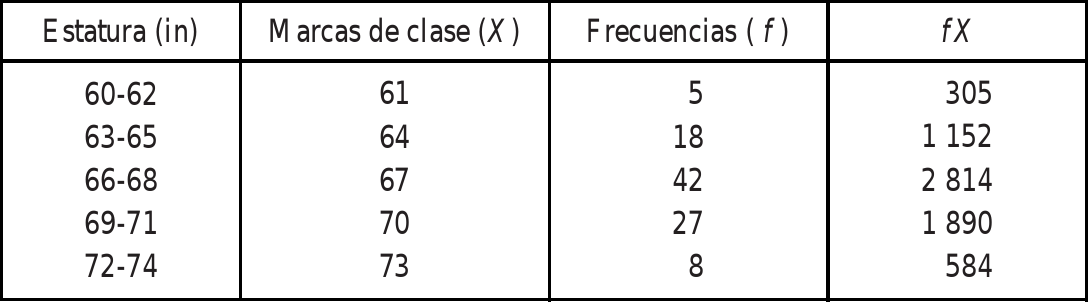
\includegraphics[width=10cm,keepaspectratio=true]{./images/tab0301.png}
  % tab0301.png: 0x0 pixel, 300dpi, 0.00x0.00 cm, bb=
  \label{tab:0301}
 \end{figure}
 \end{problema}

 

 
 \begin{problema}
 	\label{problema:3.18}
  Si las desviaciones de $N$ números $X_{1},..,X_{N}$ respecto a un \emph{pivote} $P$ están dada por $d_{i}=X_{i}-P, \; i=1,...,N$ respectivamente, demostrar que
  \begin{align}
 \bar{X}=P+\dfrac{\sum d}{N}.
 \end{align}
 \end{problema}

 
 
 \begin{problema}
 	\label{problema:3.16}
  Demostrar que la suma de las desviaciones $d_{1},d_{2},...,d_{N}$ de $X_{1},X_{2},...,X_{N}$ usando como pivote su media $\bar{X}$ es igual a cero.
 \end{problema}

 
 
 \begin{problema}
 	\label{problema:3.17}
  Si $Z_{i}=X_{i}+Y_{i}, \; i=1,2,...,N,$ demostrar que $\bar{Z}=\bar{X}+\bar{Y}.$
 \end{problema}

 

 
 \begin{problema}
  \label{problema:3.19}
  Halle la media aritmética de los números 5,8,11,9,12,6,14 y 10 eligiendo como \emph{pivote} a) $P=9$ y b) $P=20.$
 \end{problema}

 

 
  \begin{problema}
   \label{problema:3.20}
   Utilice la marca de la clase media como pivote, para calcular la estatura de los estudiantes en la tabla \ref{tab:0301}.
  \end{problema}

 
 
  \begin{problema}
   \label{problema:3.28}
   Encontrar el peso mediano a partir de la siguiente tabla
   \begin{figure}[ht]
  \centering
  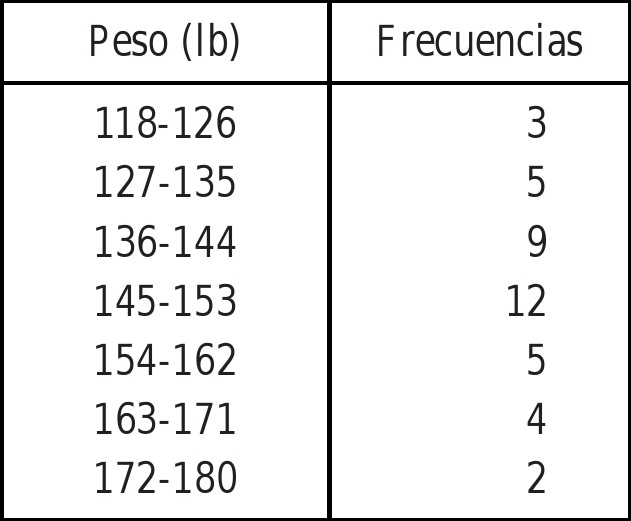
\includegraphics[height=5cm,keepaspectratio=true]{./images/tab0307.png}
  % tab0307.png: 0x0 pixel, 300dpi, 0.00x0.00 cm, bb=
  \label{tab:0307}
 \end{figure}

  \end{problema}

 

\section{Medidas de dispersión}

\paragraph{Dispersión o variación}
 Si bien las medidas de tendencia central nos dicen alrededor de que valores se concentra un arreglo de datos, las \emph{medidas de dispersión} nos dan una idea de que tan alejados están entre sí.

 



 A continuación, veremos algunas medidas de dispersión comúnmente usadas en estadística.

\paragraph{Rango}
El \emph{rango}
 de un conjunto de datos es la diferencia entre el mayor y el menor del conjunto.



\begin{ejemplo}
 El rango del conjunto 2,3,3,5,5,5,8,10,12 es $12-2=10.$
\end{ejemplo}


\paragraph{Desviación media}
La \emph{desviación media} o \emph{desviación promedio} de un conjunto de $N$ números $X_{1},...,X_{N}$ está definida como
\begin{align}
DM=\dfrac{\sum \abs{X_{j}-\bar{X}}}{N}
\end{align}
donde $\bar{X}$ es la media aritmética de los números y $\abs{\cdot}$ denota el valor absoluto.


\begin{ejemplo}
 Encuentre la desviación media de la lista $2,3,6,8,11.$
\end{ejemplo}


\paragraph{Desviación estándar}
La \emph{desviación estándar} de un conjunto de $N$ números $X_{1},...,X_{N}$ se denota como $s$ y está definida por
\begin{align}
s=\sqrt{\dfrac{\sum\left( X_{j}-\bar{X} \right)^{2}}{N}}=\sqrt{\sum\dfrac{x_{j}^{2}}{N}}
\end{align} donde $x_{j}:=X_{j}-\bar{X}.$


Si $X_{1},...,X_{N}$ se presentan con frecuencias $f_{1},...,f_{N}$ respectivamente, la desviación estándar se puede expresar como
\begin{align}
s=\sqrt{\dfrac{\sum f_{j}\left( X_{j}-\bar{X} \right)^{2}}{N}}=\sqrt{\dfrac{\sum f_{j}x_{j}^{2}}{N}}
\end{align}


 \begin{rem}
  En ocasiones, $N$ se reemplaza por $N-1$ en las fórmulas anteriores, debido a que está definición aproxima mejor a la población de la que se ha obtenido la muestra. Pero para muestras muy grandes $N>30$ prácticamente no hay diferencia.
 \end{rem}


\paragraph{Varianza}
La \emph{varianza} de un conjunto de números se define como el cuadrado $s^{2}$ de la desviación estándar $s$.


 \begin{rem}
  En estadística, es importante distinguir entre la desviación estándar de una \emph{población} y una \emph{muestra}. Para distinguirla, en el primer caso utilizaremos $\s$ y en el segundo, continuaremos usando $s.$
 \end{rem}


\paragraph{Método abreviado}
 \begin{align}
  s^{2}&=\overline{X^{2}}-\overline{X}^{2} \\
  &= E(X^2)-\left( E(X) \right)^{2}
  %\\ 
  %s^{2}&=\overline{d^{2}}-\overline{d}^{2}
 \end{align}



En las distribuciones normales se tiene que
\begin{enumerate}[(a)]
 \item $68.27\%$ de los datos está comprendido entre $\bar{X}\pm s.$
 \item $95.45\%$ de los datos está comprendido entre $\bar{X}\pm 2s.$
 \item $99.73\%$ de los datos está comprendido entre $\bar{X}\pm 3s.$

\end{enumerate}



 Si $2$ conjuntos de $N_{1}$ y $N_{2}$ datos respectivamente tienen correspondientes $s_{1}^{2}$ y $s_{2}^{2}$ varianzas pero una misma media aritmética $\bar{X},$ entonces la varianza de la unión de ambos conjuntos es
 \begin{align}
s^{2}=\dfrac{N_{1}s_{1}^{2}+N_{2}s_{2}^{2}}{N_{1}+N_{2}}.
\end{align}

\paragraph{Teorema de Chebyshev}
Para $k>1,$ por lo menos $1-\dfrac{1}{k^{2}}$ de la distribución de problemaabilidad de cualquier variable aleatoria está a nomas  de $k$ desviaciones estándar de la media.

\subsection{Python}
[]{\texttt{numpy.std}}
\begin{lstlisting}[language=Python]
numpy.std(a, axis=None, dtype=None, out=None, ddof=0,
keepdims=<class numpy._globals._NoValue>)
\end{lstlisting}

Calcule la desviación estándar a lo largo del eje especificado.

Devuelve la desviación estándar, una medida de la propagación de una distribución, de los elementos de la matriz. La desviación estándar se calcula para la matriz aplanada de forma predeterminada, de lo contrario sobre el eje especificado.\footnote{https://docs.scipy.org/doc/numpy/reference/generated/numpy.std.html}

[]
\begin{lstlisting}[language=Python]
import numpy as np

a = np.array([[1, 2], [3, 4]])
print np.std(a)
#1.1180339887498949
print np.std(a, axis=0)
#array([ 1.,  1.])
print np.std(a, axis=1)
#array([ 0.5,  0.5])
\end{lstlisting}


[]
\begin{lstlisting}[language=Python]
#In single precision, std() can be inaccurate:
a = np.zeros((2, 512*512), dtype=np.float32)
a[0, :] = 1.0
a[1, :] = 0.1
print np.std(a)
#0.45000005

#Computing the standard deviation in float64
#is more accurate:
print np.std(a, dtype=np.float64)
#0.44999999925494177
\end{lstlisting}





 \begin{problema}
 \label{problema:4.3}
  Encontrar el rango y las desviaciones media y estándar de los arreglos 
  \begin{enumerate}[(a)]
   \item $12,6,7,3,15,10,18,5$ 
   \item $9,3,8,8,9,8,9,18.$
  \end{enumerate}

  Compruebe sus resultados con \texttt{Python.}
 \end{problema}



 
 \begin{problema}
  \label{problema:4.4}
  Encontrar las desviaciones media y estándar de las estaturas de 100 estudiantes de la siguiente tabla:
  \begin{figure}[ht]
  \centering
  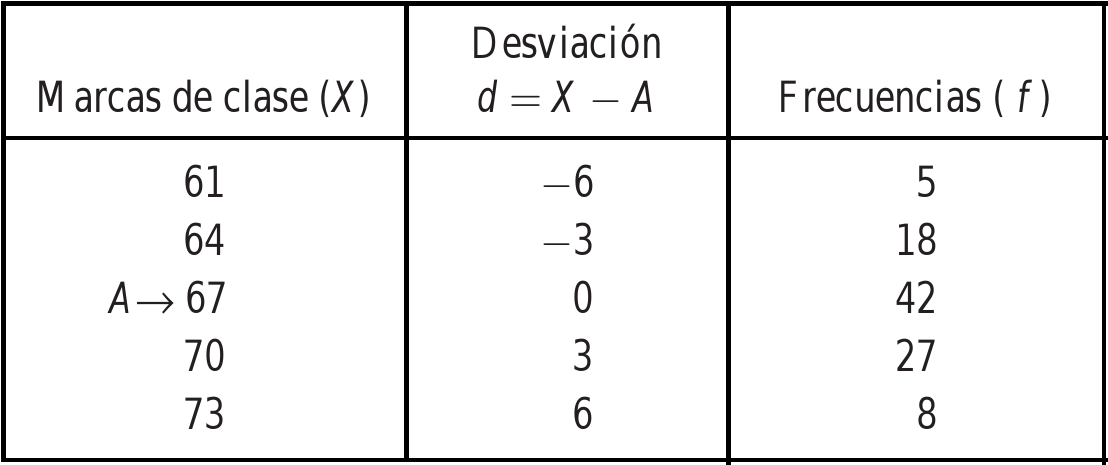
\includegraphics[width=10cm,keepaspectratio=true]{./images/tab0302.png}
  % tab0302.png: 0x0 pixel, 300dpi, 0.00x0.00 cm, bb=
  \label{tab:0302}
 \end{figure}

 \end{problema}

 

 
 \begin{problema}
  \label{problema:4.11}
  Encontrar las desviaciones media y estándar de las estaturas de 100 estudiantes de la siguiente tabla:
  \begin{figure}[ht]
  \centering
  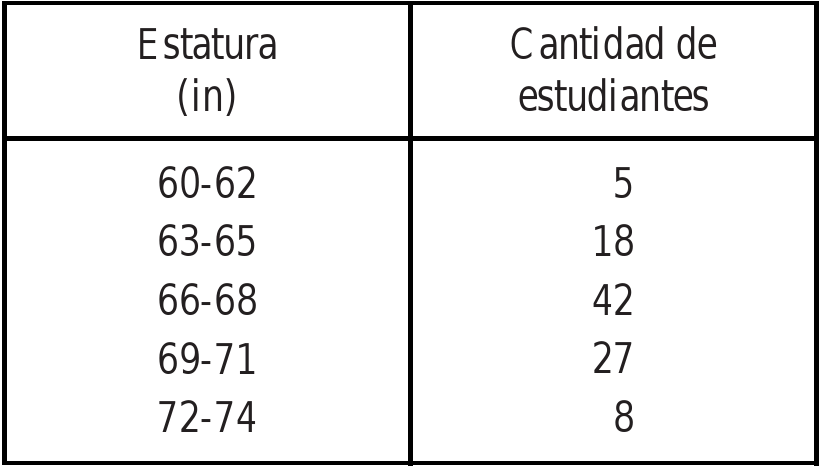
\includegraphics[height=5cm,keepaspectratio=true]{./images/tab0201.png}
  % tab0302.png: 0x0 pixel, 300dpi, 0.00x0.00 cm, bb=
  \label{tab:0201}
 \end{figure}

 \end{problema}

 

 
 \begin{problema}
  \label{problema:4.12}
  Demostrar que
  \begin{align}
 s &= \sqrt{\dfrac{\sum X^{2}}{N}-\left( \dfrac{\sum X}{N} \right)^{2}}&=
 \sqrt{\overline{X^{2}}-\overline{X}^{2}}\\
 s &= \sqrt{\dfrac{\sum fX^{2}}{N}-\left( \dfrac{\sum fX}{N} \right)^{2}}&=
 \sqrt{\overline{X^{2}}-\overline{X}^{2}}
 \end{align}
 \end{problema}

 

 
 \begin{problema}
  \label{problema:4.14}
  Utilizando las fórmulas anteriores, encuentre la desviación estándar de los datos en la tabla \ref{tab:0201}:
   \begin{figure}[ht]
  \centering
  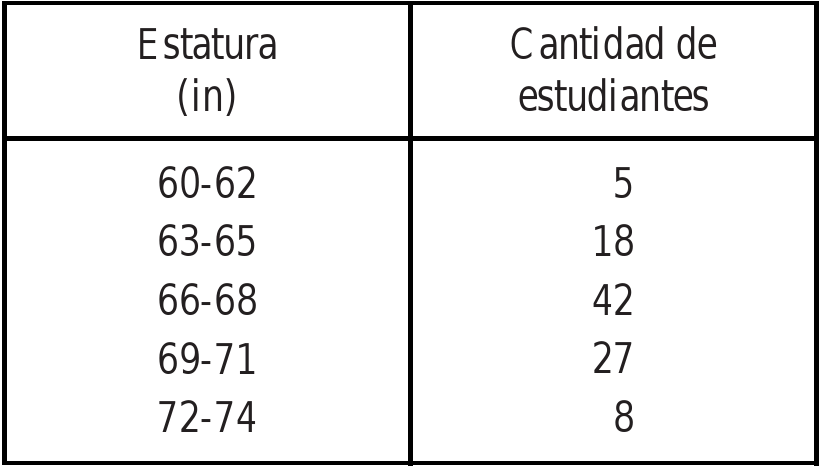
\includegraphics[height=5cm,keepaspectratio=true]{./images/tab0201.png}
  % tab0302.png: 0x0 pixel, 300dpi, 0.00x0.00 cm, bb=
  %\label{tab:0201}
 \end{figure}

 \end{problema}

 

 
  \begin{problema}
   \label{problema:4.15}
 Si $d=X-P$ son desviaciones de $X$ respecto a un pivote $P,$ demostrar que
 \begin{align}
 s=\sqrt{\dfrac{\sum fd^{2}}{N}-\left( \dfrac{\sum fd}{N} \right)^{2}}.
 \end{align}
  \end{problema}
 

 
 \begin{problema}
  \label{problema:4.17}
  Utilizando las fórmulas anteriores, encuentre la desviación estándar de los datos en la tabla \ref{tab:0201}:
   \begin{figure}[ht]
  \centering
  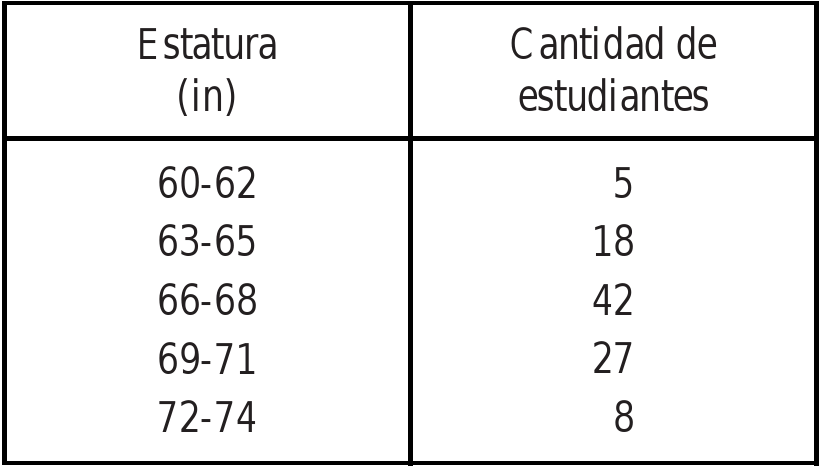
\includegraphics[height=5cm,keepaspectratio=true]{./images/tab0201.png}
  % tab0302.png: 0x0 pixel, 300dpi, 0.00x0.00 cm, bb=
  %\label{tab:0201}
 \end{figure}

 \end{problema}

 

 
  \begin{problema}
   \label{problema:4.18}
 	Encuentre la media aritmética y  la desviación estándar de los siguientes datos:
 	\begin{figure}[ht]
  \centering
  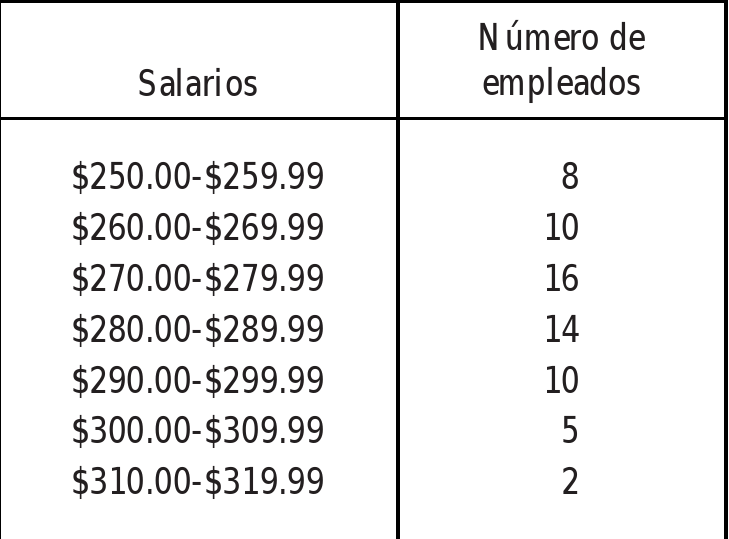
\includegraphics[height=5cm]{./images/tab0205.png}
  % tab0205.png: 0x0 pixel, 300dpi, 0.00x0.00 cm, bb=
  \label{tab:0205}
 \end{figure}

  \end{problema}
 

\section{Correlación}

 La correlación es la premisa de la modelación predictiva, en el sentido de que es un factor con base en el cuál podemos predecir resultados.


Una buena correlación entre dos variables sugiere que existe una suerte de dependencia entre ambas:  Si una cambia, la otra también lo hará. 

Podemos decir que una buena correlación asegura una relación matemática entre dos variables y debido a esto, seremos capaces de predecir su comportamiento.


La relación puede ser de cualquier tipo.  Si $x$ y $y$ son dos variables correlacionadas, entonces podemos escribir:
\begin{align}
Y=f(X)
\end{align}

\paragraph{Ejemplos de correlación}
\begin{itemize}
 \item Correlación lineal
 \begin{align}
 y = ax+b
\end{align}
\item Correlación exponencial
\begin{align}
 y = be^{ax}
\end{align}
\end{itemize}


\paragraph{Definición de correlación} Si $X,Y$ son dos variables aleatorias discretas, que pueden tomar valores $\set{x_{0},x_{1},...}$ y $\set{y_{0},y_{1},...}$, con promedios $\bar{x}, \bar{y}$  respectivamente, su correlación se define como
\begin{align}
 \corr(X,Y) = \dfrac{\sum_{x_{i},y_{j}}
 \left( \left( x_{i}-\bar{x} \right)\left( y_{j}-\bar{y} \right) \right)}
 {\sqrt{\sum_{x_{i},y_{j}}
 \left( x_{i}-\bar{x} \right)^{2}\sum_{x_{i},y_{j}}
 \left( y_{i}-\bar{y} \right)^{2}}}
\end{align}



\paragraph{Propiedades de la correlación}
\begin{itemize}
 \item El valor del coeficiente de correlación está entre $-1$ y $1$, es decir $-1\leq  \corr(X,Y)  \leq 1.$ 
 \item Una correlación positiva significa una relación directa entre las dos variables. 
 \item Una correlación negativa significa una relación inversa entre las dos variables. 
 \item Entre mayor sea la magnitud del coeficiente, más fuerte será la relación entre variables.
\end{itemize}


\paragraph{¡Advertencia!}
Aunque una correlación fuerte sugiere algún tipo de relación que puede ser utilizada para la predicción del comportamiento de una variable respecto de otra, \emph{esto no implica que dicha relación sea el único factor que explique dicho comportamiento.}


 \begin{rem}
  \emph{¡Correlación no implica causalidad!}
 \end{rem}



 Por ejemplo, existe una correlación positiva muy fuerte entre el número de palabras que conoce un ser humano y el número de calzado que utiliza...  Pero esto esto se explica porque a medida que el ser humano crece, necesita zapatos más grandes y aprende palabras nuevas. 

 \emph{¡No quiere decir que si utilizas un número más grande serás más culto!}


Tratemos de entender mejor este concepto mirando una base de datos y tratando de encontrar una correlación entre sus variables.  La base de datos que estaremos observando es una muy popular sobre los costos varios incurridos en \emph{publicidad por diferentes medios} y \emph{ventas de un producto en particular.}


Posteriormente, utilizaremos el método conocido como \emph{regresión lineal} para explorar estos mismo datos.

Por ahora, importemos esta base de datos y calculemos los coeficientes de correlación:

[,]{\texttt{advertising.py}}
\begin{lstlisting}[language=Python]
#!/usr/bin/env python3
# -*- coding: utf-8 -*-

import pandas as pd

advert = pd.read_csv("./dataBases/Advertising.csv")
print(advert.head())

import numpy as np

advert["dX*dY"] = ( advert["TV"] -
  np.mean(advert["TV"])) * ( advert["Sales"]
  np.mean(advert["Sales"]))
advert["dX**2"] = ( advert["TV"] -
  np.mean(advert["TV"])) ** 2
advert["dY**2"] = ( advert["Sales"] -
  np.mean(advert["Sales"])) ** 2

sxy = advert.sum()["dX*dY"]
sxx = advert.sum()["dX**2"]
syy = advert.sum()["dY**2"]

r = sxy/np.sqrt(sxx*syy)
\end{lstlisting}


[,]{Salida de la pantalla}
\begin{lstlisting}[language=Python]
      TV  Radio  Newspaper  Sales
0  230.1   37.8       69.2   22.1
1   44.5   39.3       45.1   10.4
2   17.2   45.9       69.3    9.3
3  151.5   41.3       58.5   18.5
4  180.8   10.8       58.4   12.9
\end{lstlisting}



[,]{\texttt{advertising2.py}}
\begin{lstlisting}[language=Python]
#!/usr/bin/env python3
# -*- coding: utf-8 -*-

import pandas as pd

advert = pd.read_csv("./dataBases/Advertising.csv")
print(advert.head())

import numpy as np

def rCoef(df, var1, var2):
    df["dX*dY"] = (df[var1]-np.mean(df[var1]))*(df[var2]-np.mean(df[var2]))
    df["dX**2"] = (df[var1]-np.mean(df[var1]))**2
    df["dY**2"] = (df[var2]-np.mean(df[var2]))**2
    sxy = df.sum()["dX*dY"]
    sxx = df.sum()["dX**2"]
    syy = df.sum()["dY**2"]
    r = sxy/np.sqrt(sxx*syy)
    return r

tvVsSales = rCoef(advert, "TV", "Sales")
## 0.782224424862
radioVsSales = rCoef(advert, "Radio", "Sales")
## 0.576222574571
\end{lstlisting}




\begin{figure}[h]
 \centering
 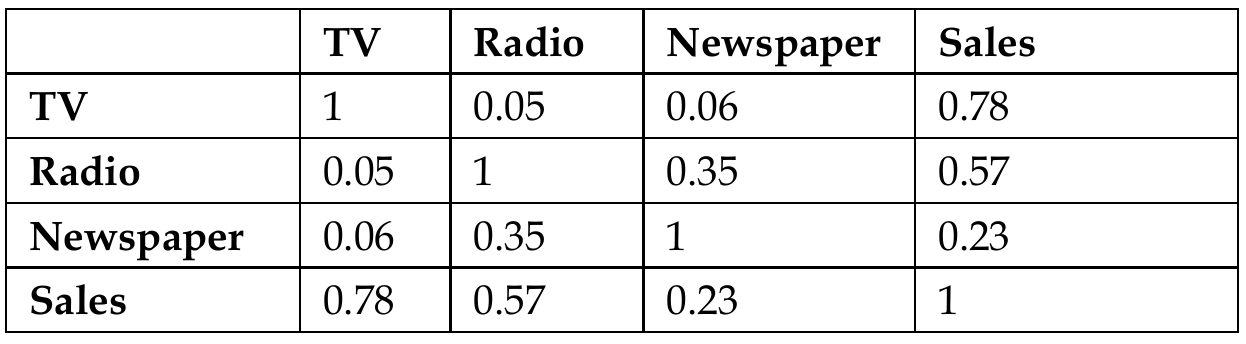
\includegraphics[width=10cm,keepaspectratio=true]{./images/correlationMatrix.png}
 % correlationMatrix.png: 0x0 pixel, 300dpi, 0.00x0.00 cm, bb=
 \caption{Matriz de correlación}
 \label{correlationMatrix}
\end{figure}



Veamos la naturaleza de esta correlación graficando las variables \texttt{TV}, \texttt{Radio} y \texttt{Newspaper} vs \texttt{Sales} del \textit{data frame} \texttt{advert}.

[,]{tvVsSales.py}
\begin{lstlisting}[language=Python]
#!/usr/bin/env python3
# -*- coding: utf-8 -*-

import pandas as pd
advert = pd.read_csv("./dataBases/Advertising.csv")

import matplotlib.pyplot as plt

plt.plot(advert['TV'],advert['Sales'],'ro')
plt.title('TV vs Sales')
plt.show()

plt.plot(advert['Radio'],advert['Sales'],'ro')
plt.title('Radio vs Sales')
plt.show()

plt.plot(advert['Newspaper'],advert['Sales'],'ro')
plt.title('Newspaper vs Sales')
plt.show()
\end{lstlisting}


\begin{center}
 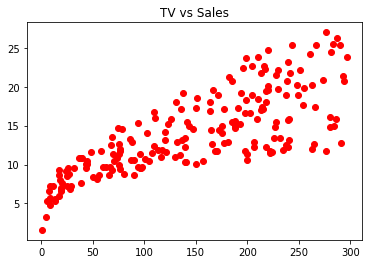
\includegraphics[width=10cm,keepaspectratio=true]{./images/tvVsSales.png}
 % tvVsSales.png: 0x0 pixel, 300dpi, 0.00x0.00 cm, bb=
\end{center}


\begin{center}
 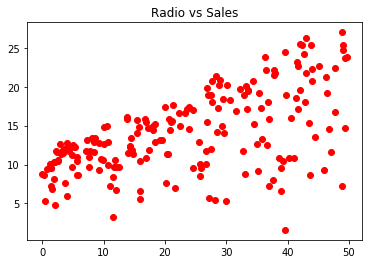
\includegraphics[width=10cm,keepaspectratio=true]{./images/radioVsSales.png}
 % tvVsSales.png: 0x0 pixel, 300dpi, 0.00x0.00 cm, bb=
\end{center}


\begin{center}
 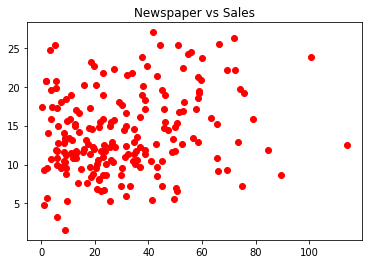
\includegraphics[width=10cm,keepaspectratio=true]{./images/newsVsSales.png}
 % tvVsSales.png: 0x0 pixel, 300dpi, 0.00x0.00 cm, bb=
\end{center}

